\documentclass[nobib]{MSword}
% Class options:
%-------------------------------
% nobib         - skip bibliography code/ don't include bib
% math          - include math packages and useful math commands
% hidelinks     - hide hyperref colored link boxes
% wordlinks     - link color scheme similar to word


% Preamble code:
%%%%%%%%%%%%%%%%%%%%%%%%%%%%%%%%%%%%%%%%
\usepackage[english]{babel}
\usepackage{csquotes}
\usepackage{lipsum}

% % Uncomment using "Ctrl + /" (/ on numpad):
% % Customizing headers and footers:
% \fancypagestyle{custom}{%
%     \fancyhf{}% clears the footer and header
%     % Header:
%     \fancyhead[L]{}
%     \fancyhead[C]{}
%     \fancyhead[R]{}
%     % Footer:
%     \fancyfoot[L]{}
%     \fancyfoot[C]{}
%     \fancyfoot[R]{}
%         % Tips:
%         % ----
%         % L: left, C: center, R: right
%         % O: odd pages, E: even pages
%         % ----
%         % Example: \fancyghead[LO,RE]{Text}
%         % will produce "Text" left in the header
%         % on odd pages and right in the header on even pages.
%     % Rules/ lines:
%     \renewcommand{\headrulewidth}{0.4pt}
%     \renewcommand{\footrulewidth}{2pt}
% }
% % Changing the pagestyle:
% \pagestyle{custom}

%%%%%%%%%%%%%%%%%%%%%%%%%%%%%%%%%%%%%%%%

% Preamble information:
%%%%%%%%%%%%%%%%%%%%%%%%%%%%%%%%%%%%%%%%

\title{Filter Design}
\author{Dre Mata}
\date{24 April 2023}

%%%%%%%%%%%%%%%%%%%%%%%%%%%%%%%%%%%%%%%%

% The document:
%%%%%%%%%%%%%%%%%%%%%%%%%%%%%%%%%%%%%%%%
\begin{document}

\maketitle
\begin{center}
    Introduction
\end{center}
The objective of this lab is to design a band pass filter for a fictional scenario. The scenario is that we are instructed by our boss to design a filter that can be used to filter out noise for an airplane's position sensor. There are many other signals causing noise for the position sensor and it is our job to filter out all the other noises. The position sensor has a frequency of 1.8kHz to 2.0kHz. All other frequencies are to be treated as noise that needs to be filtered. 

\begin{center}
    Task 1:
\end{center}
The first task for this lab was to identify noise magnitudes and corresponding frequencies of low and high frequency noise. This was done by using the fast Fourier transform function that was created in a previous lab. Once the input signal was transformed I graphed the whole signal to get an idea of what it looked like. Then I graphed the low frequency noise and then I graphed the high frequency noise to get an idea of what the noise signal looks like. The graphs for the whole fft, low frequency noise, and high frequency noise can be seen in graphs 1-3 respectively. I then graphed the position sensors frequency. This can be seen in graph 4.

\begin{center}
    Task 2 and 3:
\end{center}
The second task was to create a band pass circuit to filter out the noise of the signal. I decided to choose my capacitor value first and calculate other values around it by using the band width and center frequency. The once the values were found I used python to graph a bode plot of the transfer function for my values, but I saw that it was still filtering out some of the position sensor. I then changed the resistance value until the bode plot was appropriate for the signal. The diagram and values for the band pass filter can be seen in Figure one. The transfer function can be seen in Figure two. The bode plot for the filter can be seen in Graph five. It can be seen in the bode plot that the position measurement information is attenuated less than -0.3dB, low frequency noise is attenuated by -30dB, switching amplifier noise is attenuated by -21dB, and no noise over 100kHz exist. 

\begin{center}
    Task 4:
\end{center}
The fourth and final task of this project was to then use the filter that was designed in task 2 to filter out the appropriate frequencies in the input. The output of this signal can be seen in graph six.

\begin{center}
    Questions:
\end{center}

1. Earlier this semester, you were asked what you personally wanted to get out of taking this
course. Do you feel like that personal goal was met? Why or why not?

My goal was to learn practical knowledge in this class and I feel that this goal was met. I have been interning at SEL this semester, and I have used many concepts from this class in my internship. It helps me see how this information is used in the real world. Also this lab has helped with my python skills greatly.

\begin{center}
    Figures
\end{center}

Graph 1:

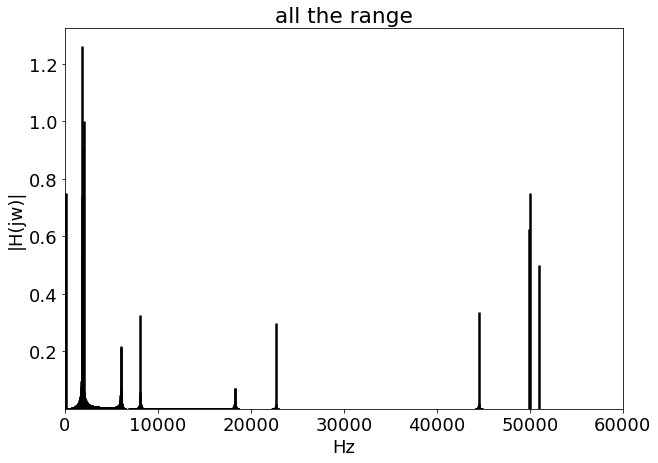
\includegraphics[scale = 0.6]
{txt/Lab12GraphAll.png}

Graph 2:

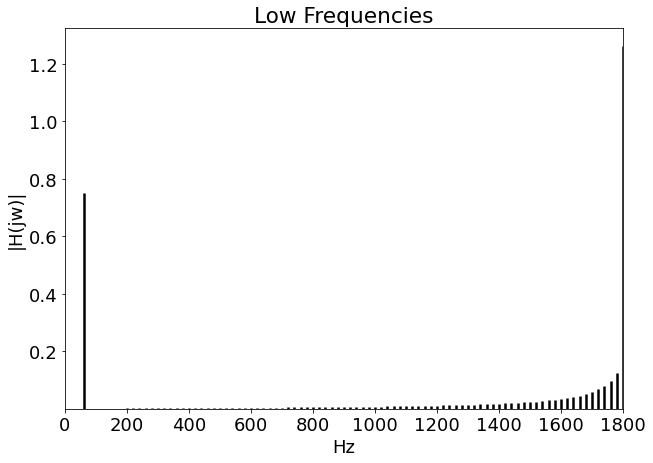
\includegraphics[scale = 0.6]
{txt/Lab12Graph2.png}


Graph 3:

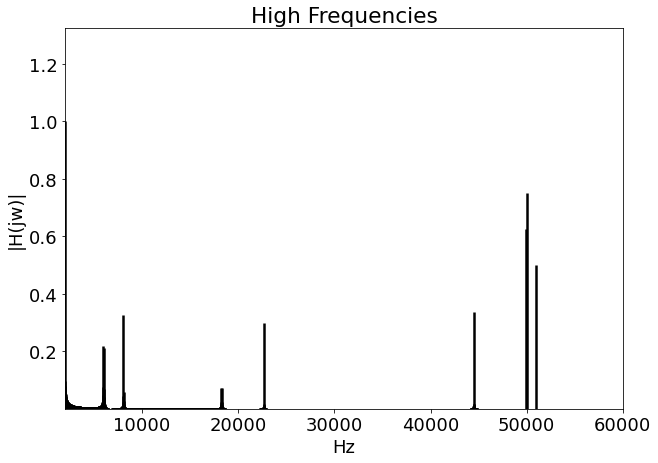
\includegraphics[scale = .6]
{txt/Lab12Graph3.png}

Graph 4:

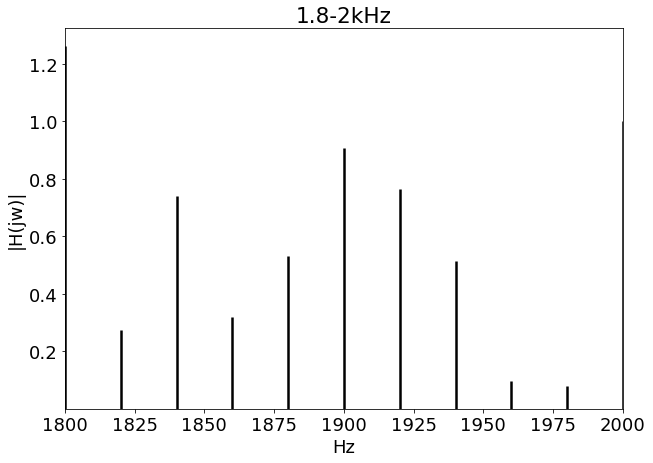
\includegraphics[scale = 0.6]
{txt/Lab12Graph4.png}

Graph 5:

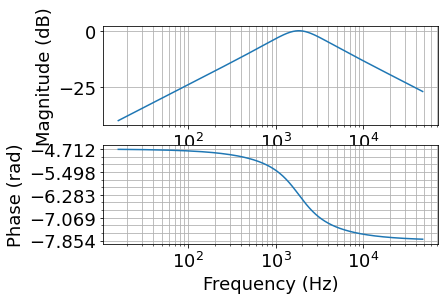
\includegraphics[scale = 0.8]
{txt/Lab12Graph5.png}

Graph 6:

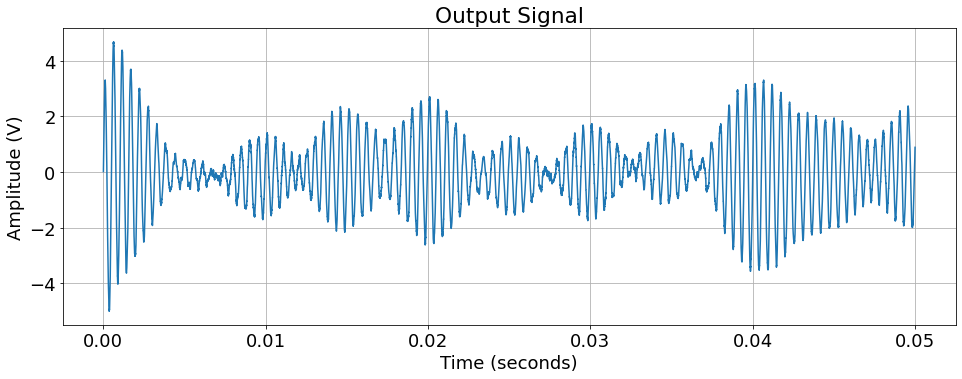
\includegraphics[scale = 0.4]
{txt/Lab12Graph6.png}

Figure 1:

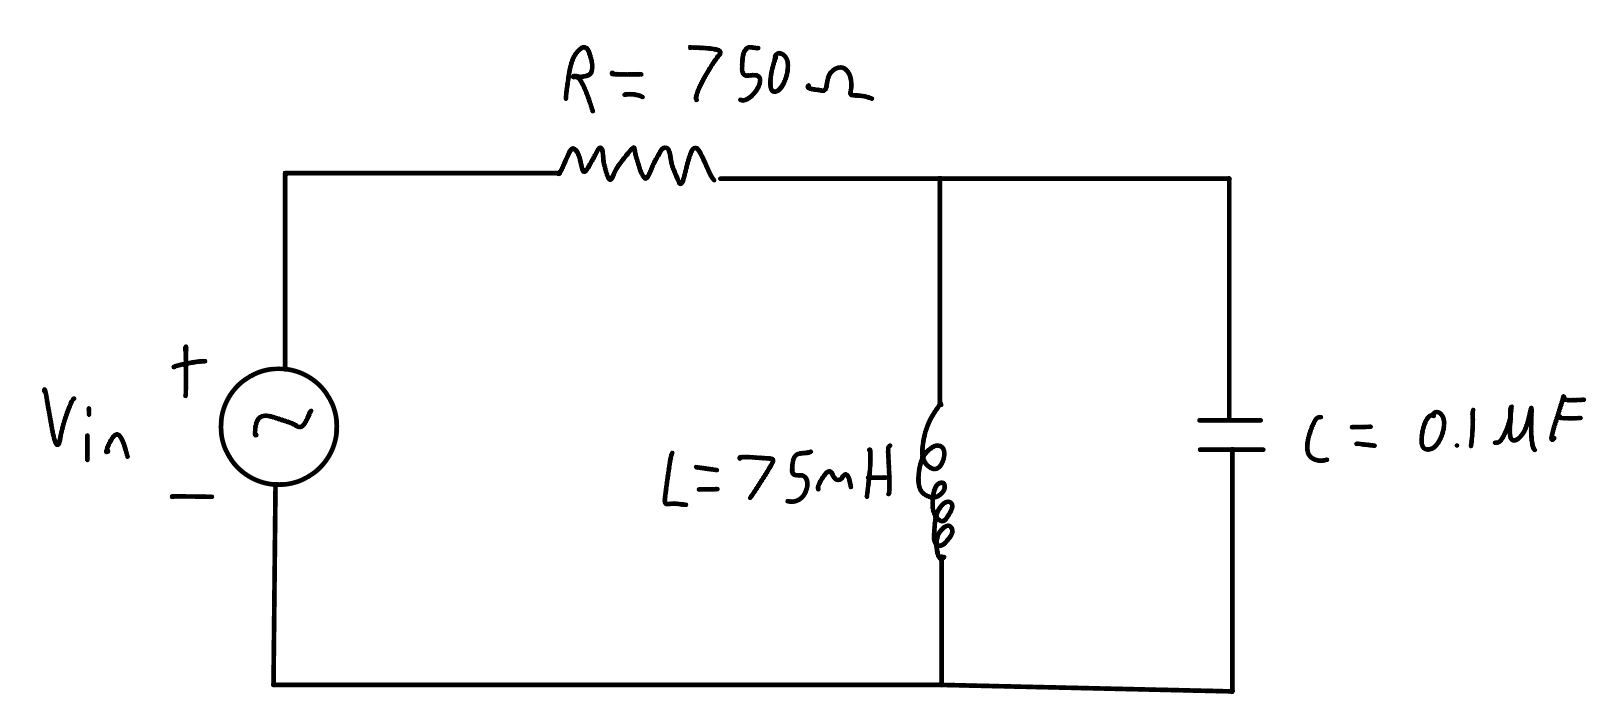
\includegraphics[scale = 0.2]
{txt/Lab12Figure1.jpeg}

Figure 2:

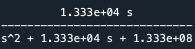
\includegraphics[scale = 1]
{txt/Lab12Figure2.png}

\begin{center}
    Conclusion
\end{center}
I enjoyed this lab, because it felt that I know what needed to be done and I was given vague instructions on how to do it. So I was able to go through a process that made sense to me without having to adhere to rigid instructions. It was also nice that it used many concepts from over the semester, so a lot of the code was able to be transferred over. It was also satisfying to see the end result of the lab and how a filter is critical in signals like these.
\end{document}
%%%%%%%%%%%%%%%%%%%%%%%%%%%%%%%%%%%%%%%%

% Copyright Remarks:
%--------------------

% Copyright holder: Vebjørn S. Førde, copyright: CC BY 4.0
% Note: The author of this template is also the copyright holder.

% Below is an explanation of the CC BY 4.0. Additional statements/ 
% clarifications made by the author/copyright holder are marked with *.

% YOU ARE FREE TO:
% Share — copy and redistribute the material in any medium or format
% Adapt — remix, transform, and build upon the material
% for any purpose, even commercially.

% UNDER THE FOLLOWING TERMS:
% Attribution* — You must give appropriate credit, provide a link to the license,
% and indicate if changes were made. You may do so in any reasonable manner, but 
% not in any way that suggests the licensor endorses you or your use.

% *Note: 
% Attribution NOT NEEDED for: 
%       - PDF distibution (like sharing your PDF document)
%       - Use of (dummy)text and images provided in the template (obviously)
%       - Distributing parts of the template, and not the template as a whole
% I am not really concerned with being given credit. As long as you do not 
% claim to have made the template yourself in distributing it further, I have
% no complaints.

% No additional restrictions — You may not apply legal terms or technological 
% measures that legally restrict others from doing anything the license permits.

% NOTICES:
% No warranties are given.

% Disclaimer* (added by copyright holder):
% THE SOFTWARE IS PROVIDED "AS IS", WITHOUT WARRANTY OF ANY KIND, EXPRESS OR
% IMPLIED, INCLUDING BUT NOT LIMITED TO THE WARRANTIES OF MERCHANTABILITY,
% FITNESS FOR A PARTICULAR PURPOSE AND NONINFRINGEMENT. IN NO EVENT SHALL THE
% AUTHORS OR COPYRIGHT HOLDERS BE LIABLE FOR ANY CLAIM, DAMAGES OR OTHER
% LIABILITY, WHETHER IN AN ACTION OF CONTRACT, TORT OR OTHERWISE, ARISING FROM,
% OUT OF OR IN CONNECTION WITH THE SOFTWARE OR THE USE OR OTHER DEALINGS IN THE
% SOFTWARE.

% Read more about CC BY 4.0:
% https://creativecommons.org/licenses/by/4.0/